\section{Introduction}

Humans readily acquire skills from open-ended instructions and feedback from others
\citep{tomasello1993cultural}. These instructions and feedback are internalized for
self-regulated learning \citep{pintrich2002development,nicol2006formative}, providing
internal signals for continuous improvement. Drawing inspiration from this
process, we investigate how well AI agents can benefit from open-ended human feedback
through induction of generalizable metrics.

We can characterize existing evaluations and rewards for AI agents into two main
classes: (1) goal-oriented evaluation -- \emph{whether the agents have fulfilled
the given task}, \emph{e.g.} benchmarks \citep{zhouwebarena,jimenezswe,chan2024mle,paglieri2024balrog}
and reward modeling approaches \citep{pan2024autonomous,chen2025scaling,choudhury2025process}
and (2) behavior evaluation -- \emph{the manner the agents perform the task}, \emph{e.g.}
social agent and human-agent interaction benchmarks \citep{zhousotopia,shao2024collaborative}
and agent failure mode analysis \citep{pan2025why,zhang2023effects,yang2023behavioral}.\footnote{Note
that the difference between the two classes is not whether the evaluation is
based on the outcome or the process. Both evaluations can be performed at every step
or in the final step.} Goal-oriented evaluation is often designed to be
verifiable, but is not sufficiently fine-grained or comprehensive to diagnose agents'
behavior problems or locate improvement bottlenecks \citep{yehudai2025survey}.
Although the above can be complemented with behavior evaluation, it requires manual
design of metrics based on top-down heuristics \citep{zhousotopia}, or thematic analysis
of the agent's behavior \citep{shao2024collaborative,pan2025why}. This manual design
process requires the labor of experts in annotations and classification, which
limits its scalability.

In this paper, we introduce AutoLibra \protect
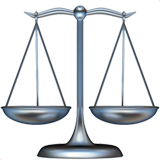
\includegraphics[height=1em]{figs/scale.png}
, a metric induction method, as a novel agent evaluation framework that
mitigates the limitations of current evaluation paradigms. AutoLibra is an evaluation
tool that induces interpretable metrics for AI agents from open-ended human feedback,
which can be collected from end users of AI agents or experts. This offers two key
advantages: (1) It is much easier to provide concrete feedback for trajectories
than creating metrics, and (2) AutoLibra allows us to evaluate agents from the perspective
of the users. AutoLibra-induced metrics provide concrete definitions of
behaviors that the model-based evaluation method should look for when evaluating
AI agents, which could be used to understand agent behavior, as well as
optimization targets to improve agents.

Inspired by the code-theme steps of thematic analysis conducted by experts in
social sciences \citep{braun2006using}, we design the AutoLibra induction
process (\S\ref{sec:induction_process}) as two steps: (1) \emph{feedback
grounding}: where we ground every aspect of human feedback on some behavior in
the entire agent trajectory, and (2) \emph{behavior clustering}: where we cluster
the aspects into multiple clusters of similar behaviors to summarize into metrics.
As illustrated in Fig. \ref{fig:teaser}, the user gives a web agent feedback ``the
agent did not choose iPhone 14/15'' which is grounded to the agent's behavior, choosing
``iPhone 16 Pro'' from the drop-down menu. Similar behaviors are clustered into
a common cluster, summarized as \textit{Element Interaction Accuracy}.

\begin{figure}[!t]
	\centering
	\includegraphics[width=0.86\linewidth]{figs/autolibra_teaser_v2.pdf}
	\caption{AutoLibra \protect
	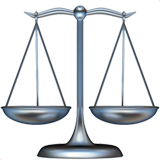
\includegraphics[height=1em]{figs/scale.png}
	induces agent evaluation metrics from human feedback, and uses these metrics to
	evaluate agents, which can be meta-evaluated via evaluating the coverage on
	unseen human feedback. Here we show real examples of agent trajectories, human
	feedback, aspects, induced metrics, evaluation results on WebVoyager \citep{he2024webvoyager}.}
	\label{fig:teaser}
\end{figure}

The AutoLibra evaluation process is designed to provide a closed-loop feedback signal
for the induction process. The agent trajectories used in the induction process
are scored by LLM-as-a-Judge \citep{zheng2023judging} on the induced metrics.
The evaluation process (\S\ref{sec:evaluation_process}) then tries to match the feedback
aspects, \emph{e.g.} ``recipe does not contain quinoa'', with the traits, \emph{e.g.}
\texttt{task-requirement-achievement}. In this way, we can meta-evaluate the quality
of the metrics: (i) \emph{coverage} (what proportion of feedback aspects can be
matched with an agent trait), and (ii) \emph{redundancy} of the metrics (what
proportion of the detected traits are not mentioned by humans). These two
metrics provide an overall statistical picture of the quality of the induced
metrics. Based on these two metrics, we can search for the set of metrics with
the lowest redundancy within those with the highest coverage. As shown in \S\ref{sec:metric-optimization},
we find that as the number of metrics increases, the redundancy increases, and the
coverage ultimately converges to the maximum coverage.

With AutoLibra, our aim is to answer the following research questions:

\begin{description}
	\item[\textbf{RQ1:}] How aligned are the results from AutoLibra for each step with
		human judgment?

	\item[\textbf{RQ2:}] Can AutoLibra provide more insight into agent behavior that
		were not provided by expert designed metrics?

	\item[\textbf{RQ3:}] Can AutoLibra provide optimization signals for human agent
		engineers and agent learning algorithms to improve agents' performance?
\end{description}

\textbf{Key findings:} Experiments within multiple agent domains, including collaborative
agents \citep{shao2024collaborative}, social agents \citep{zhousotopia}, web agents
\citep{zhouwebarena,he2024webvoyager}, and text game agents \citep{paglieri2024balrog,cloos2024babaaibreakrules},
demonstrate that AutoLibra is able to induce fine-grained and interpretable metrics
with high coverage and low redundancy in unseen human feedback with 80 trajectories
annotated with one feedback for each trajectory per dataset. These metrics are
more concrete, and some of them were even overlooked in expert designed metrics or
error analysis (\S\ref{sec:lens}). The fact that AutoLibra can iteratively discover
new, emergent metrics (\S\ref{sec:iterative-induction}) throughout the agent optimization
process, and provide salient and human-interpretable optimization signals helps
improve the performance in Baba-Is-AI by over 20\% (\S\ref{sec:Baba-Is-AI}), and
web-browsing task WebVoyager by 5\% on top of previous model-based rejection
fine-tuning methods (\S\ref{sec:webvoyager}) with only 18 trajectories annotated
with one feedback for each trajectory in each improvement iteration.

% \diyi{i think the Introduction still needs some work. First, why do we even want to do metric induction? Why can't we ask humans to come up with metrics? Why do we prefer to let humans provide feedback into the process, and then induce the metrics from it? It is okay to start with cons of existing metrics, but then we need to discuss how we should mitigate issues of prior evaluation metrics. We want to leverage human feedback because it is easier for humans to provide natural language feedback in terms of how the agent is doing, compared to asking humans to design metrics. Such procedural metrics give more insights compared to an overall task level signal. I don't know whether we want to draw any connections of these metrics derived by autolibra compared to behavior or goal oriented metrics, as it might be possible that some of these are behavior while others could be indicative of goals.}